%%%%%%%%%%%%%%%%%%%%%%%%%%%%%%%%%%%%%%%%%%%%%%%%%%%%%%%%%%%%%%%%%%%%%%%%%%%%%%%%%%%%%%%%%%%%%%%%%%%
% Chapter 5 -> Methods for TI
% Author: Mingbo Cheng
%%%%%%%%%%%%%%%%%%%%%%%%%%%%%%%%%%%%%%%%%%%%%%%%%%%%%%%%%%%%%%%%%%%%%%%%%%%%%%%%%%%%%%%%%%%%%%%%%%%
%\addbibresource{~/MEGA/MEGAsync/phd/thesis_Cheng/preamble/thesis.bib}
\chapter{Methods for Trajectory Inference}
\label{chapter:methods_TI}
\graphicspath{{chapter5/figs}}

In the previous two chapters, we presented the implementation of single-cell integration methods and the benchmarking to validate our MOJITOO method. With a shared latent space, we can further perform several downstream analyses, among which trajectory inference is crucial for capturing cell differentiation. Inferring trajectories is challenging since we can only capture specific time points of single cells rather than the dynamic process. Trajectory inference for single-cell multimodal data provides an opportunity to delve deeper into biological processes.

This chapter exclusively introduces the formalization and implementation of our novel trajectory inference method for single-cell multimodal data. We first introduce the necessary notation for the method (\sref{TI_methods:notation}). Next, we present the implementation details of trajectory inference, specifically focusing on graph triangulation, Hodge decomposition, and tree creation (\sref{TI_methods:TI}). Following that, we describe the implementation details of our package (\sref{TI_methods:implementation}). Finally, we conclude this chapter by discussing the strengths of our method (\sref{TI_methods:discussion}).


\section{Notation} \label{TI_methods:notation}

$D: $ Diagonal matrix of a graph\\
$W: $ Kernel(Affinity) matrix \\
$M: $ Transition matrix \\
$\mathcal{V}: $ A set of vertices\\
$\mathcal{S}^k = \{{v}_0,\cdots,{v}_k \}: $ A $k$-simplex\\
$\mathcal{X}: $ A simplicial complex.\\
$\mathcal{C}_k(\mathcal{X}): $ Vector space with coefficients in $\mathbb{R}$ whose basis is the set of oriented k-simplices of $\mathcal{X}$\\
$\partial_k ([v_0,\cdots, v_k])$: boundary map\\
$\mathbf{B}_k: $ A k order incidence matrix.\\
$L_0: $ Zero-order Graph Laplacian\\
$L_1: $ Hodge 1-Laplacian\\
$\mathcal{L}_1: $ Normalized Hodge 1-Laplacian\\
$\mathcal{L}_1^S: $ Symmetrized Normalized Hodge 1-Laplacian\\
\section{Trajectory Inference}
\label{TI_methods:TI}



\subsubsection{Diffusion Map}

Given a common cell joint embedding $X^l$, we represent the data as a diffusion map~\citep{coifman2005geometric}. For this, we first estimate a Gaussian kernel $W$:
\begin{equation}
\label{eqn:gussiankernel}
W_{ij} = \exp\left({-\frac{\|x_i^l - x_j^l\|^2}{\sigma_i \sigma_j}}\right)
\end{equation}
\noindent where $x^l_i$ is the representation of sample (cell) $i$ in the embedding $X^l$ and $\sigma_i$ is the local scaling parameter. This is estimated with the distance to the $n$-th nearest neighbor from $x^l_i$ as in \cite{zelnik2004self}.

\noindent The (zero-order) Graph Laplacian $L_0$ can be defined as:
\begin{equation}
\label{eqn:L0}
L_0 = D - W
\end{equation}
\noindent where $D$ is a diagonal matrix that the $i$-th entry $d_{ii} = \sum_j W_{ij}$.  The random walk on graph laplacian $L_0$ we can reach the steady state~\citep{delvenne2010stability} where
\begin{equation}
\label{eqn:transitionmatrix}
p_{t+1} = p_t D^{-1}W \equiv p_t M
\end{equation}

\noindent where $p_t\in \mathbb{R}^n$ is normalized probability vector, $M$ is transition matrix of the graph. Next, we perform eigendecomposition on the symmetric form of $M$ such that:
\begin{equation}
\label{eqn:l0symeigendecomposition}
M' = D^{\frac{1}{2}}(M) D^{-\frac{1}{2}} = D^{\frac{1}{2}}(D^{-1}W) D^{-\frac{1}{2}} = D^{-\frac{1}{2}}WD^{-\frac{1}{2}} = Q\Lambda Q^\top
\end{equation}

\noindent Taking advantage of the above eigen-decomposition, we can effectively calculate $M^s$ (see~\cite{coifman2005geometric}), such that:
\begin{equation}
\label{eqn:l0eigendecomposition}
    M^s = (D^{-\frac{1}{2}} M' D^{\frac{1}{2}})^s =  (D^{-\frac{1}{2}} Q\Lambda Q^\top D^{\frac{1}{2}})^s =  D^{-\frac{1}{2}} Q \Lambda^s Q^\top D^{\frac{1}{2}}
\end{equation}
Where $D^{-\frac{1}{2}}Q$ columns includes the right eigen vectors of $M$ and rows of $Q^\top D^{\frac{1}{2}}$ includes the left eigen vectors. Diagonal matrix $\Lambda$ contains the corresponding eigenvalues.

% XXX - what is M^s. Define how this is estimated from eq. 4.  --fixed
Finally, we can estimate pseudotime $u$ (or potential) at time $t=s$ as:
\begin{equation}
\label{eqn:potential}
u = (1/m, 1/m,\cdots, 1/m, 0,0,\cdots,0)M^{s}
\end{equation}
\noindent where $m$ is the number of start cells, and $s$ is the diffusion process at the time $t=s$.


\subsection{Graph based pseudotime estimation}

To improve the pseudotime estimates, we use a procedure similar to~\cite{maehara2019ddhodge}, which smooths pseudo-time estimates by considering the graph connectivity. For this, we define initial edges weights as gradient values of the fully connected graph, e.g. $w^{F}_{ij}=u_j - u_i$. Next, we prune this fully-connected graph by considering only the $k$ nearest-neighbors. This provides a graph $G^{(knn)}=(\mathcal{V}, \mathcal{E})$, where $\mathcal{V}$ is the set of vertices and $\mathcal{E}$ is the set of edges.
We represent this graph as an incidence matrix $\mathbf{B_1}$. For an edge $e_i \in \mathcal{E}$ and vertex $v_j \in \mathcal{V}$, we have:
\begin{equation}
\label{eqn:incidencematrix}
\mathbf{B}_1[i,j] = \begin{cases}
-1 &\text{if edge } e_i \text{ leaves  vertex }v_j \\
1 &\text{if edge } e_i \text{ enters  vertex }v_j \\
0 &\text{if otherwise}.
\end{cases}
\end{equation}
This is used to define the incidence matrix for full graph and pruned $k$-nn graph respectively $\mathbf{B_1}^F$ and $\mathbf{B_1}^P$.
\noindent We want to estimate pseudo-times of the pruned $k$-nn graph by using the pseudo-time estimates of the full graph. For this, we get a first estimate of the gradients of the truncated graph ($w^P$) by minimizing:
\begin{equation}
\label{eqn:transitionmatrix}
    \min_{w}\frac{1}{2}\|\mathbf{B_1}^F w^F - \mathbf{B_1}^P w^P\|^2 + \frac{\lambda}{2}\|w^P\|^2,
\end{equation}
\noindent where $\lambda$ is the regularization parameter. Next, we update the potential of the vertices
\begin{equation}
  u' = \arg\underset{u'}{\min}\|(\mathbf{B_1}^P)^\top u' - w^P\|^2.
\end{equation}
\noindent This allows us to estimate an updated gradients $w^s=\mathbf{B_1}^\top u'$. Next, we use these gradients to estimate the final pseudotime $u^s$ of the vertices as:
\begin{equation}
    u^s = \arg\underset{u^s}{\min} \| \mathbf{B_1}^\top u^s - w^s\|^2.
\end{equation}
\noindent With the graph $G^{(knn)}$ with edge weights $w^s$ and pseudotime estimates $u^s$, we estimate a diffusion embedding with the kamada-kawai layout algorithm~\citep{gansner2004graph, ortmann2016sparse}. Examples of the graph layouts and pseudo-time estimates can be seen in~\afref{supfig:fib2neuron-workflow}A.

\subsection{Hodge Laplacian Decomposition on a Single Cell Simplicial Complex}

Given $G^{(knn)}$ and pseudo-time estimate $u^s$, the next steps are the creation of a simplicial complex and estimation of the Hodge Laplacian decomposition.

\subsubsection{Triangulated Single cell graph}

A typical cell differentiation graph has tree-like structures. Laplacian decomposition are able to find distinct type of topological structures (connected components, holes, voids), but not trees or branches. We resort to a simple trick, i.e. it uses pseudo-time estimates to find end-state cells and adds dummy/artificial edges from end-state to start state cells.  This creates holes in the data, one for each trajectory in the tree. For this, we obtain $m$ (default 5) cells with highest and lowest pseudotime. We include directed edges from terminal (high pseudotime) to start (low pseudo-time) vertices. Next, we use a Delaunay triangulation~\citep{delaunay1934bulletin} on the diffusion embedding to create uniformly distributed set of triangles around the single cell graph by first ignoring the dummy edges. Next, we remove edges connecting distant cells, i.e. we estimate the distribution of distance of connected vertices and obtain the value associated with the 75$\%$ quantile ($Q_{75}$) and we remove all edges connecting vertices, which distance is higher than $3\times Q_{75}$. We further refine the dummy eddges by performing a triangulation between each pair of terminal cells and root cells. This results in a triangulated graph $G^{(t)} = (\mathcal{V}^{(t)},\mathcal{E}^{(t)},\mathcal{T}^{(t)})$, where $\mathcal{V}^{(t)}$ is the vertices set, $\mathcal{E}^{(t)}$ is the edge set of graph $G^{(t)}$ and $\mathcal{T}^{(t)}$ is the set of triangles. A triangle can be loosely defined as a 3-vertex clique, i.e. a set of tree fully connected by edges. An example of the simplex representation of a differentiation tree is provided in~\afref{supfig:fib2neuron-workflow}B.


\subsubsection{Simplicial Complex}
A $k$-simplex~\citep{schaub2021signal}~(\fref{fig:simplex}) $\mathcal{S}^k = \{{v}_0,\cdots,{v}_k \}$ is an unordered subset of a finite set of vertices $\mathcal{V}$ with cardinality $k + 1$, where $v_i\in \mathcal{V}$, $v_i \neq v_j$ and $i \neq j$.

\begin{figure}[!h]
    \centering
    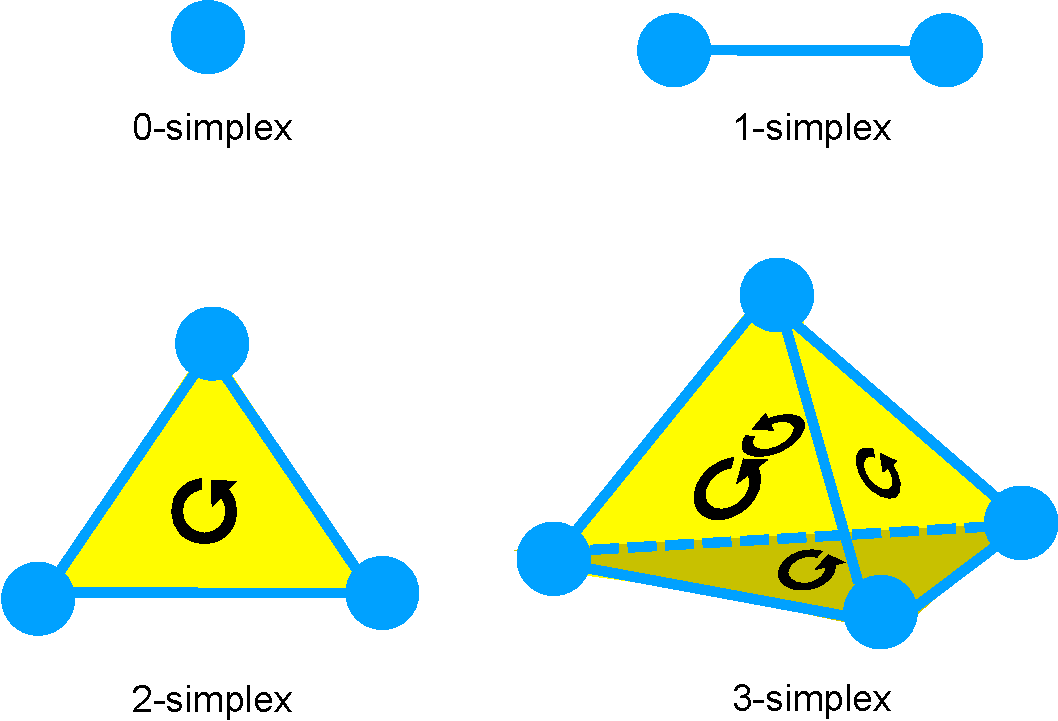
\includegraphics[width=0.45\textwidth]{Simplex/fig}
    \vspace{0.1cm}
    \caption[0-simplex to 3-simplex.]{0-simplex to 3-simplex.}
    \label{fig:simplex}
\end{figure}

A simplicial complex~(SC)~(\fref{fig:sc}) $\mathcal{X}$ is a collection of simplices, where for all $k$-simplices $\mathcal{S}^k$ in $\mathcal{X}$, any subset of $\mathcal{S}^k$ must also be in $\mathcal{X}$. The typical $0$-simplices, $1$-simplices, $2$-simplices are also respectively called vertices, edges and triadic faces. A face of a simplex $\mathcal{S}^k$ is a subset of $\mathcal{S}^k$  with cardinally $k$ in the form $\{v_0 \cdots v_{i-1}, v_{i+1}\cdots v_k\}$ for $0 \leq i \leq k$. A co-face $\mathcal{S}^{k+1}$ of a simplex $\mathcal{S}^k$ is a $(k + 1)$-simplex such that $\mathcal{S}^k$ is a subset of $\mathcal{S}^{k+1}$.  When ordering vertices of a $k$-simplex $\{{v}_0,\cdots,{v}_k \}$, it becomes an orientated $k$-simplex denoted by $[{v}_0,\cdots,{v}_k ]$, where the orientation changing corresponds to the change of sign of the coefficient, i.e. $[{v}_0,\cdots {v}_i, \cdots {v}_j\cdots,{v}_k ]$ = $-[{v}_0,\cdots {v}_j, \cdots {v}_i\cdots,{v}_k ]$.

\begin{figure}[!h]
    \centering
    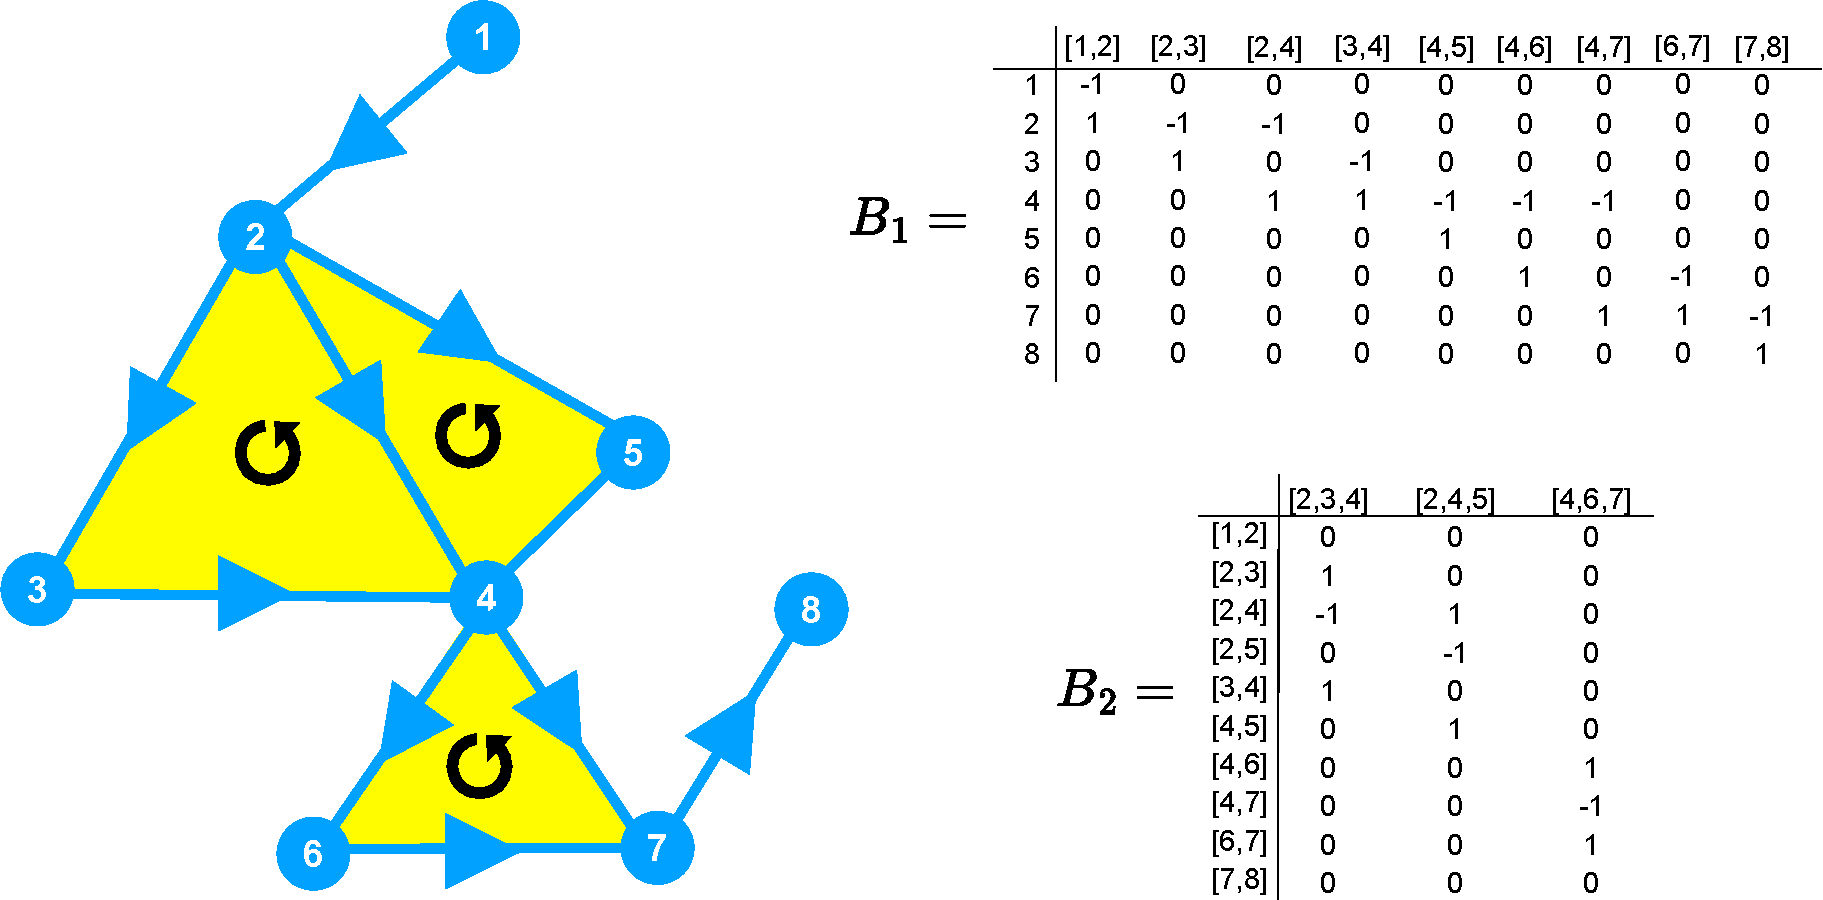
\includegraphics[width=0.65\textwidth]{Simplicial_Complex/fig}
    \vspace{0.1cm}
    \caption[A simplicial complex example.]{Example of a ordered simplicial complex and boundary maps $\mathbf{B}_1$ and $\mathbf{B}_2$ representing this
complex.}
    \label{fig:sc}
\end{figure}


For each $k \geq 0$, $\mathcal{C}_k(\mathcal{X})$ is the vector space with coefficients in $\mathbb{R}$ whose basis is the set of oriented k-simplices of $\mathcal{X}$. $\mathcal{C}_k(\mathcal{X}) = 0$ when $k$ is larger than the dimension of $\mathcal{X}$. An element of these vector spaces $c_k \in \mathcal{C}_k(\mathcal{X})$ is called a $k$-chain, which is a linear combination of the basis elements. The boundary map is defined as the linear transformations $\partial_{k}$: $\mathcal{C}_k(\mathcal{X}) \rightarrow \mathcal{C}_{k-1}(\mathcal{X})$ acts on basis elements as follows:
\begin{equation}
\partial_k ([v_0,\cdots, v_k]) = \sum_{i=0}^{k} (-1)^i [v_0, \cdots, v_{i-1}, v_{i+1}, \cdots, v_k]
\end{equation}
$\mathrm{im}(\partial_k)$ is the space of $(k-1)$-boundaries, where $\mathrm{im}(.)$ is the image of an operator. We can construct the matrix representation of the boundary operators $\partial_k$ by $\mathbf{B}_k$~\citep{lim2020hodge,muhammad2006control}. 

%For example, as shown in~\fref{fig:sc}, the incidence matrices $\mathbf{B}_1$ and $\mathbf{B}_2$ of the 2-simplicial complex capture the relationships between nodes and edges, and edges and triangles, respectively.

Specifically, for a given triangulated graph $G^{(t)}$, a next task is to obtain a second order simplicial complex (SC). These can be represented by the estimation of incidence matrices, or boundary operations $\mathbf{B}_k$ which maps $k-1$ simplices to $k$ simplices. For example, $\mathbf{B}_1$ captures the relation between vertices (0-simplices) and edges (1-simplices) and $\mathbf{B}_2$ captures the relation between edges (1-simplices) and triangles (2-simplices)~\citep{schaub2021signal}~\frefp{fig:sc}.
%A simplicial complex is a set composed of vertices ($0$-simplices), edges ($1$-simplices) and triangles ($2$-simplices) and their $k$-dimensional counterparts

The boundary matrix on 1-simplices $\mathbf{B}_1$ is defined as in \eref{eqn:incidencematrix}. An entry in $\mathbf{B}_2$ capturing the relationship between an directed edge $e_i \in \mathcal{E}$ and a directed triangle $\bigtriangleup_{q} \in \mathcal{T}$ can be defined as:
\begin{equation}
\label{eqn:incidencematrix}
\mathbf{B}_2[i,q] = \begin{cases}
-1 &\text{if }e_i \in \bigtriangleup_{q} \text{ and } e_i \text{ has same direction as the triangle}\bigtriangleup_{q}  \\
1 &\text{if }e_i \in \bigtriangleup_{q} \text{ and } e_i \text{ has opposite direction than the} \bigtriangleup_{q} \\
0 &\text{if otherwise}.
\end{cases}
\end{equation}

Check figure \ref{fig:sc} for an example of a simplicial complex and its corresponding $\mathbf{B}_1$ and $\mathbf{B}_2$ matrices. There we can find several edges ($[1,2]$, $[2,3]$, $[2,4]$, $[2,5]$, $[3,4]$, $[4,5]$, $[4,6]$, $[4,7]$, $[6,7]$, $[7,8]$) and  3 triangles ($[2,3,4]$, $[2,4,5]$ and $[4,6,7]$). Entry $B_1 [1,1]$ has value -1, as the first edge $e_1=(1,2)$ leaves vertex $1$, while $\mathbf{B}_1[2,1]$ has value 1, as the first edge $[1,2]$ enters the vertex $2$. Regarding $\mathbf{B}_2$, all entries related to the first edge  $e_1=(1,2)$ are zero, as there is no triangle associated to it. $\mathbf{B}_2[2,1]$ is equal to one as the direction of  $e_2=(2,3)$ fits the direction of the first triangle ($\bigtriangleup_1=(2,3,4)$). $\mathbf{B}_2[3,1]$ is equal to -1 as the third edge ($e_3=(2,4)$) has opposite direction to $\bigtriangleup_1=(2,3,4)$. We refer the reader to~\citep{Schaub2020} for a in depth characterization of simplicial complexes.

Here, we are only interested in the direction of edges (flows) and the direction of triangles are only used for book keeping, i.e. their directions follow the index of the vertices in increasing order. Note also that the boundary operation requires less memory than adjacency matrices for sparse graphs, i.e. $\mathbf{B}_1$ is smaller than a graph incidence matrix if the number of edges is smaller than the number of vertices. A similar rational follows for $\mathbf{B}_2$.


\subsubsection{Hodge Laplacian and decomposition}

Hodge Laplacian is a higher order generalized form of graph Laplacian, for a graph $G$, The $k$-th hodge Laplacian is:
\begin{equation}
\label{eqn:hodgeLaplacian}
{L}_k = \mathbf{B}_{k}^\top \mathbf{B}_{k} + \mathbf{B}_{k+1} \mathbf{B}_{k+1}^\top
\end{equation}
where $\mathbf{B}_k$ is the incidence matrix.

For $k=0$, ${L}_0$ is the same as the zero order graph Laplacian introduced in \eref{eqn:graphLaplacian}..
\begin{equation}
\label{eqn:graphLaplacian}
{L}_0 =  \mathbf{0}^\top  \mathbf{0} + \mathbf{B}_{1} \mathbf{B}_{1}^\top =  \mathbf{D}_1 - \mathbf{A},
\end{equation}
\noindent where $\mathbf{D}_1$ is the diagonal matrix of a graph and $\mathbf{A}$ is the adjacency matrix.

Here, we are interested in the first order Hodge Laplacian, i.e.:
\begin{equation}
\label{eqn:hodgeLaplacian}
{L}_1 = \mathbf{B}_{1}^\top \mathbf{B}_{1} + \mathbf{B}_{2} \mathbf{B}_{2}^\top.
\end{equation}
As in diffusion maps~\citep{witten1981diffusion}, it is preferable to work with the normalized form of the Hodge Laplacian, as this provides a random walk process on the simplex~\citep{Schaub2020}:
\begin{equation}
\label{eqn:normL1}
\mathcal{L}_1 = \mathbf{D}_2 \mathbf{B}_1^\top \mathbf{D}_1^{-1} \mathbf{B}_1 + \mathbf{B}_2 \mathbf{D}_3 \mathbf{B}_2^\top \mathbf{D}_2^{-1}
\end{equation}
\noindent where $\mathbf{D}_2$ is the diagonal matrix of (adjusted) degrees of each edge, i.e. $\mathbf{D}_2 = \max{(\text{diag}(|\mathbf{B}_2| \mathbf{1}), \mathbf{I})}$. $\mathbf{D}_1$ is the diagonal matrix of weighted degrees of the vertices, and $\mathbf{D}_3=\frac{1}{3}\mathbf{I}$. Like the standard form of $\mathcal{L}_0$, here $\mathcal{L}_1$ is asymmetric which makes eigen-decomposition hard. To address this, we construct the symmetric form of $\mathcal{L}_1$ as following:
\begin{equation}
\label{eqn:normL1sym}
\mathcal{L}_1^s = \mathbf{D}_2^{-1/2} \mathcal{L}_1 \mathbf{D}_2^{1/2} = \mathbf{D}_2^{1/2} \mathbf{B}_1^\top \mathbf{D}_1^{-1} \mathbf{B}_1 \mathbf{D}_2^{1/2} + \mathbf{D}^{-1/2} \mathbf{B}_2 \mathbf{D}_3 \mathbf{B}_2^\top \mathbf{D}_2^{-1/2}.
\end{equation}
\noindent Next, we perform eigendecomposition on the symmetric form $\mathcal{L}_1^s$ such that:

\begin{equation}
\label{eqn:l1symeigendecomposition}
\mathcal{L}_1^s = Q\Lambda Q^\top
\end{equation}
\noindent where columns of $Q$ are the eigenvectors and the diagonal elements of the diagonal matrix $\Lambda$ indicate the corresponding eigenvalues. Thus the decomposition of the normalized form $\mathcal{L}_1$ becomes:
\begin{equation}
\label{eqn:l1decomposition}
\mathcal{L}_1 = \mathbf{D}_2^{1/2} \mathcal{L}_1^s \mathbf{D}_2^{-1/2} =  \mathbf{D}_2^{1/2} Q \Lambda Q^\top \mathbf{D}_2^{-1/2} = \mathbf{U} \Lambda \mathbf{U}^{-1}
\end{equation}
\noindent where $Q\in \mathbb{R}^{\|\mathcal{E}^{(t)})\|\times \|\mathcal{E}^{(t)})\|}$ is the eigenvector of $\mathcal{L}_1^s$, $\|\mathcal{E}^{(t)})\|$ is the number of edges in graph $G^{(t)}$, the diagonal matrix $\Lambda\in \mathbb{R}^{\|\mathcal{E}^{(t)})\|}$ records the corresponding eigenvalues. We can make use of the right eigenvector $q_R = \mathbf{D}_2^{1/2} q$ as the edges spectrum.

For example, for the embryonic mouse data, we observe that the Harmonic decomposition has two eigenvalues close to zero. If we plot the harmonic values for these two eigenvectors in the vertices, we observe that they highlight the two major branches of the triangulated graph~(\afref{supfig:fib2neuron-workflow}C). This is equivalent to the spectral clustering algorithm, where spectra (and small eigenvalues) are associated with the number of disconnected components (or clusters) in a graph.
%~(\afref{supfig:L0-L1}).

\subsubsection{Determining the number of harmonic functions}
In practice, the harmonic functions corresponding to eigenvalues are not exactly zero. Therefore, it's better to determine the number of harmonics automatically. We developed a simple algorithm for this purpose. The idea is straightforward: since the eigenvalues are already ordered, we can check the division of each eigenvalue with the previous one. It's easy to detect a jump, which indicates that the current eigenvalue is significantly larger than the previous one. In \fref{fig:breakingpoint}, we can see that the division values range from 0 to 3 in all cases except for the 11 eigenvalues, where the division is \num{3.05e+12}. Thus, we detect the top 10 eigenvectors as the harmonic functions. For details on the implementation of the detection algorithm, refer to \alref{alg:breaking_point}.

\begin{figure}[!ht]
    \centering
    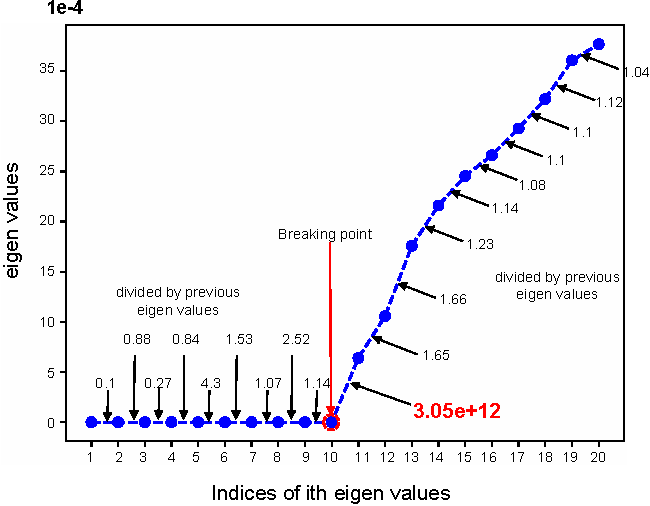
\includegraphics[width=0.65\textwidth]{breakingpoint/fig}
    \vspace{0.1cm}
    \caption[Number of eigens selecting algorithm.]{\textbf{Number of eigens selecting algorithm.} The eigenvalues are derived from the benchmarking data, specifically from the Diffusion Limited Aggregation Tree with 10 branches.}
    \label{fig:breakingpoint}
\end{figure}

\begin{algorithm}
    \Input{
        $\textbf{x}$, indices of eigen values\\
        $\textbf{y}$, eigen values\\
    }
    \Output{
        $\text{index}$, the indice of the break point
    }
    $L_{div} \gets ()$ \Comment*[r]{division list}
    \While{$i \in \textup{\textbf{x}}(2:)$}{
        $L_{div}(i) \gets \left|\frac{\textbf{y}(i)}{\textbf{y}(i-1)}\right|$ \Comment*[r]{divided by the previous element}
    }
    $\text{index} \gets \arg\max_{\forall i \in \textbf{x}(2:)} L_{div}(i)$\\
    $\text{index} \gets \text{index}-1$ \Comment*[r]{the previous index is the breaking point}

    \Return{$\textup{\text{index}}$}
    \caption{Breaking point detecting algorithm}
    \label{alg:breaking_point}
\end{algorithm}

\subsection{Trajectory Embedding and Tree Inference}

\subsubsection{Trajectory Sampling}

To generate trajectories, we sample paths (or edge flows) in the graph by following edges with positive divergence (or increasing pseudotime).  Due to the sparsity of the triangulated graph $G^{(t)}$, we sample paths in $G^{(knn)}$. For this, we perform a preference random walk on graph $G^{(knn)}$. We choose a random starting point from vertices (cells) with $m$ lowest pseudo-time values. We choose the next vertex randomly by considering the divergence values ($w^s$). Only positive divergences (increase in pseudo-time) are considered. We stop when no further positive potential is available. Next, we return to the triangulated graph $G^{(t)}$ and estimate shortest paths in case sampled edges (from $G^{(knn)}$) are not present in $G^{(t)}$. We define a path $\mathbf{f}\in\mathbb{R}^{\|\mathcal{E}^{(t)}\|}$ on a simplicial complex as:
\begin{equation}
    \mathbf{f}[i,j] = \begin{cases}
        1\quad & \text{if edge }(i,j) \text{ is traversed}\\
        -1\quad & \text{if edge }(j,i) \text{ is traversed}\\
        0 \quad & \text{otherwise}
    \end{cases}
\label{eq:edgeflow}
\end{equation}
Random walk is repeated $n$ times. This provides us with a path matrix $\mathbf{F}^{(t)}\in \mathbb{R}^{\|\mathcal{E}^{(t)}\| \times n}$, where $\|\mathcal{E}^{(t)}\|$ is number of edges in graph $G^{(t)}$. See~\afref{supfig:fib2neuron-workflow}D for examples of sampled trajectories or edge flows. For details on the implementation of the random walk, refer to \alref{alg:randomwalk}. 

\begin{algorithm}
    \Input{
        $A$, Adjacency matrix\\
        $W$, Diffusion distance matrix\\
        $G^{t}=\{\mathcal{V}^{t},\mathcal{E}^{t}\}$, Triangulated graph\\
    }
    \Parameter{
        $N$, Number of trajectories\\
        $K=9$, KNN graph using A, W\\
        $\text{pct}$, Percentage of starting cells\\
    }
    \Output{
        $L_p$, The list of trajectories\\
    }

    $i \gets 1$ \\
    $G^{knn}=\{\mathcal{V}^{knn}, \mathcal{E}^{knn}\} \gets \textbf{Graph}(A,W,K)$ \\
    $\mathcal{V}_{low}^{knn} \gets \textbf{LowestPseudotime}(\mathcal{V}^{t}, \text{pct})$ \Comment*[r]{pct is percentage parameter}
    $U[v] \gets \textbf{PesudoTime}(v)$ \Comment*[r]{Pseudo time of node v}
    $L_p \gets (()_{1}, ()_{2}, \cdots ()_{N})$\Comment*[r]{List of list}
    \While{$i \leq N$}
    {
        $l_{temp} \gets ()$ \\
        $\text{node} \gets \textbf{random}(\mathcal{V}_{low}^{knn})$ \\
        $l_{temp} \gets \textbf{Append}(l_{temp}, \text{node})$ \\
        \While{$\textup{\textbf{true}}$}{
            $\text{NextNodes} \gets \{\mathcal{V} | \mathcal{V}\in \textbf{Neighbor}(\mathcal{E}^{knn}, \text{node}) \text{ and } U[\mathcal{V}]>U[\text{node}]  \}$\\
            \If{$\textup{NextNodes} == \emptyset$}{
                \textbf{break}
            }
            $\text{NextNode} \gets \textbf{PropRandom}(\text{NextNodes})$ \\
            $l_{temp} \gets \textbf{Append}(l_{temp}, \text{NextNode})$ \\
            $\text{node} \gets \text{NextNode}$\\
        }
        $\text{Len} \gets \textbf{Length}(l_{temp})$\\
        $k \gets 1$\\
        \While{$k < \textup{Len}$}{
            $\text{node}_a \gets l_{temp}(k)$\\
            $\text{node}_b \gets l_{temp}(k+1)$\\
            \If{$(\textup{node}_a, \textup{node}_b) \in \mathcal{E}^{t}$}{
                $\text{NodeList} \gets \textbf{ShortestPath}(G^{t}, \text{node}_a, \text{node}_b)$\\
                $L_p(i) \gets \textbf{Append}(L_p(i), \text{node}_a)$\\
                $L_p(i) \gets \textbf{Extend}(L_p(i), \text{NodeList})$\\
            }\Else{
                $L_p(i) \gets \textbf{Append}(L_p(i), \text{node}_a)$\\
            }
        }
        $L_p(i) \gets \textbf{Append}(L_p(i), l_{temp}(\text{Len}))$\\
        $i \gets i+1$\\
    }
    \Return $L_p$
    \caption{Random walk on triangulation graph}
    \label{alg:randomwalk}
\end{algorithm}

\subsubsection{Trajectory embedding and clustering}

We next project these paths $\mathbf{F}^{(t)}$ onto harmonic space to estimate a trajectory embedding. Let's recapitulate the decomposition of the normalized Hodge 1-Laplacian~\erefp{eqn:l1decomposition}:
\begin{equation}
\mathcal{L}_1 = \mathbf{U}\Lambda \mathbf{U}^{-1},
\end{equation}
\noindent where $\mathbf{U}=(\mathbf{u}_1,\cdots, \mathbf{u}_{\|\mathcal{E}^{(t)}\|})$ is the eigenvector matrix and $\Lambda = \mathrm{diag}(\lambda_1,\cdots, \lambda_{\|\mathcal{E}^{(t)}\|})$ are the eigenvectors. We assume the eigenvectors have been sorted by their corresponding increasing eigenvalues such that $0\leq\lambda_1\leq\lambda_2\leq\cdots\leq\lambda_{\|\mathcal{E}^{(t)}\|}$.

Denote $\mathbf{H}:=(\mathbf{u}_1,\cdots, \mathbf{u}_{k})$ to be the matrix containing all the harmonic functions associated to $\mathcal{L}_1$, i.e. all of the eigenvectors corresponding to the $0$ eigenvalues, where $k$ is the number with eigenvalues being equal to 0 and $\mathbf{H}\in \mathbb{R}^{\|\mathcal{E}^{(t)}\|\times k}$. We further project edge flow matrix $\mathbf{F}^{(t)}$ onto the harmonic space by matrix multiplication  such that
\begin{equation}
\mathbf{H}^{(t)} = \mathbf{H}^\top \mathbf{F}^{(t)}
\end{equation}
where $\mathbf{H}^{(t)}\in \mathbb{R}^{k\times n}$ embed each trajectory into k dimensions. We next perform clustering on $\mathbf{H}^{(t)}$ with DBSCAN~\citep{ester1996dbscan} to group the paths into major differentiation trajectories. For the mouse embryonic cell data, we observe that the trajectory embedding (or trajectory map) reveals two clusters~(\afref{supfig:fib2neuron-workflow}E) (left) associated with the neuronal and myocyte differentiation.


\subsubsection{Cumulative trajectory embedding and tree inference}

The path representation presented in \eref{eq:edgeflow} do not keep the time step of a edge visit.  Thus we also define a traversed edge flow (transversed path) matrix $\hat{\mathbf{f}}\in \mathbb{R}^{{\|\mathcal{E}^{(t)}\|}\times S}$ to record both the time step associated with every edge visit, i.e.:
\begin{equation}
    \hat{\mathbf{f}}[i,j, s] = \begin{cases}
        1\quad & \text{if edge }(i,j) \text{ is traversed in step } s\\
        -1\quad & \text{if edge }(j,i) \text{ is traversed in step } s\\
        0 \quad & \text{otherwise}
    \end{cases}
\end{equation}
\noindent where $S$ is the length of the flow and $\|\mathcal{E}^{(t)}\|$ is number of edges in graph $G^{(t)}$. As we have $n$ trajectories, we will have $n$ traversed edge flow matrices $\{\hat{\mathbf{f}}_1, \hat{\mathbf{f}}_2,\cdots, \hat{\mathbf{f}}_n\}$.

We make use of cumulative trajectory embedding to represents paths and for detection of major trajectories and branching points. For a path $\hat{\mathbf{f}}$, we can estimate a point associated with every step $s$ in this cummulative trajectory embedding space as:
\begin{equation}
    \mathbf{v}_s =  \sum_{i = 1}^{s} \mathbf{H}^\top \hat{\mathbf{f}}_{,i}
\end{equation}
where $\hat{\mathbf{f}}_{,i}\in \mathbb{R}^k$, $k$ is the number of harmonic functions. That is,  $\mathbf{v}_s \in \mathbb{R}^k$ is a coordinate in cumulative trajectory embedding space associated to the $s$ step in trajectory $\hat{\mathbf{f}}$.  This is repeated for all step sizes, which defines a vector $\mathbf{v} = \{\mathbf{v}_1, \cdots,\mathbf{v}_S\}$ for every path. As observed in~\afref{supfig:fib2neuron-workflow}E, these vectors are low dimensional representations of paths in the cumulative trajectory embedding. By coloring paths from distinct groups with distinct colors, we can recognize branching point events, branches shared by trajectory groups and terminal branches. Note also that if we consider only the final entry for every path, we obtain the same result as in the previously described trajectory embedding.

\begin{figure}[!ht]
    \centering
    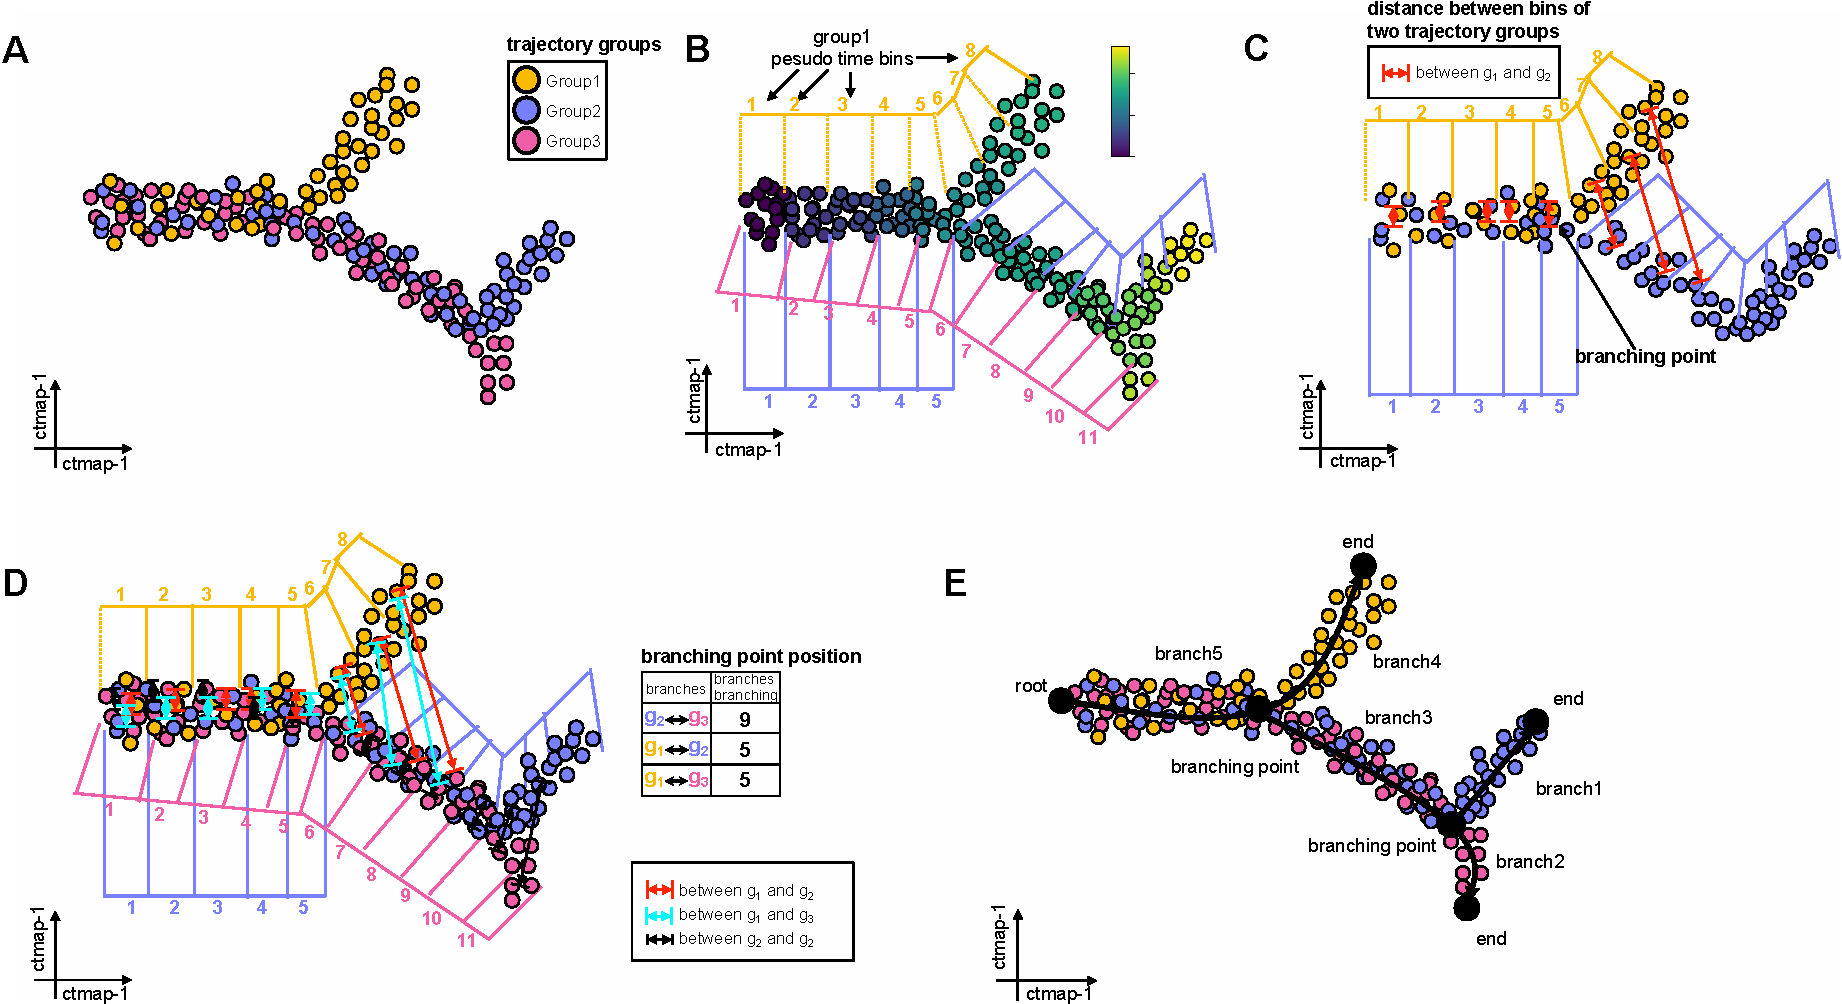
\includegraphics[width=0.65\textwidth]{branching/fig}
    \vspace{0.1cm}
    \caption[Schematic showing how to create a differentiation tree.]{\textbf{Schematic showing how to create a tree using edges lay in cumulative trajectory space.}  \textbf{A)}Example of three trajectory groups g1 , g2 , g3 each with a distinct color in the cumulative trajectory space. Every dot in this embedding represents a edge in the graph (or a cell differentiation event). \textbf{B)} We take the mean on the pseudo-time of the vertices (cells) connected by an edge and use this an the edge pseudo-time estimate. We next bin the edges by considering their pseudo-times. \textbf{C)} It then estimate average edge locations for every bin, which serves as a backbone for the trajectories. It also estimate distance between edges in two groups but with the same bin index. \textbf{D)} Distance between bins are estimated for all groups and branchings points are detected whenever distance between edges in two groups surpasses the distances of edges within a group for a given bin In the example, bin 9 is a branching point between groups 2 and 3 and bin 5 is a branching point between groups 1 and 2 and 1 and 3. \textbf{E)} To build the final tree, We consider the branching points with the highest values towards the lowest values to build trees in a bottom-up approach, i.e. it merges trajectory 2 and 3 at bin 9. The next branching point is 5, which connects trajectory 1 with the tree formed by 2 and 3.}
    \label{fig:branching}
\end{figure}

Recall that we have performed the DBSCAN clustering method to cluster the $n$ paths into $m$ groups $\{g_1, g_2, \cdots g_m\}$ on the trajectory embedding. We next use a procedure schematized in~\fref{fig:branching} to find the differentiation tree structure. First, it estimates pseudo-time values for every edge, i.e. the average pseudo-time $u^s$ from vertices associated to the edge. It next bins all edges by considering their pseudo-time, i.e. it selects the trajectory group with lowest pseudo-time and splits it edges in $p$ bins~(\fref{fig:branching} B). The same range of pseuudo-time is used to bin all trajectory groups and bins are indexed in increasing pseudo-time~(\fref{fig:branching} C).  After binning of edges for each group, We next find the branching points for all group pairs by comparing the distance of edges within the bin vs. the distance of edges between the bins for a given bin index $i$.

More formally, for groups $g_i$ and $g_j$ and bin $k$, their corresponding edges in cumulative space are defined as set $\mathbf{V}^k_i$, $\mathbf{V}^k_j$. We then estimate average edge coordinate per bin to serve as backbones for every group, i.e.:
\begin{equation}
    \overline{b^k_i} = \frac{1}{M}\sum_{v \in \mathbf{V}^k_i } v,
\end{equation}
where $M=|\mathbf{V}^k_i|$ is the number of edges in the bin. We also consider the average distance between edges in a bin to have an estimate of the compactness of edges in a bin and trajectory, i.e.:
\begin{equation}
    \overline{\sigma^k_i} = \frac{1}{M^2} \sum_{u \in \mathbf{V}^k_i}  \sum_{v \in \mathbf{V}^k_i} \Big\|u-v\Big\|_2 \qquad.
\end{equation}
Finally, we calculate the distance between two groups $g_i$ and $g_j$ in time bin $k$, such that:
\begin{equation}
    \mathrm{d}(i,j,k) = \Bigg\| \frac{ \overline{b^k_i} }{ \overline{\sigma^k_i}} - \frac{ \overline{b^k_j} }{ \overline{\sigma^k_j}} \Bigg\|_2.
    \label{eqn:dijk}
\end{equation}
For every pair of groups, We find a unique branching point by transversing bins in decreasing order and finding the first bin such that $\mathrm{d}(i,j,k) < \sigma$ (as default $1$).
% XXX - what is the value here?
This is repeated for all pairs of groups. The tree is finally built in a bottom up manner. We first consider branching points with highest index and builds a sub-tree by merging the two trajectory groups at hand. This is repeated until all branching points are considered~(\fref{fig:branching}D-F). We finally define the leaves and the root by finding more extreme points, edges with lowest and highest pseudo-time in a trajectory group. These are the so called milestones (branching points, root and end points) needed for evaluation by Dynverse~\citep{saelens2019comparison}. Trajectories are redefined as branches, i.e. part of the trajectories between two milestones. We also allocate cells (vertices) to these branches. For this, we consider the location of all edges associated with a vertex and use the mean value in the cumulative trajectory embedding space. This is used to allocate cells to branches and to find the distance between respective milestones. Moreover, we provide this information for STREAM~\citep{chen2019stream} for visualization as an STREAM tree. For detail of the tree creating procedure, refer to \alref{alg:treecreating}.


\begin{algorithm}
    \Input{
     $V = \{V_1, V_2,\cdots, V_m\}$ ,cumsum coordinates for each group; \\
     $t = \{t_1, t_2,\cdots, t_m\}$ ,group pseudo time; \\
    }
    \Parameter{
     $min_{bin}=10$ ,shortest trajectory minimum bin size; \\
     ${\theta}_{cut} = 1$ ,branching point cut distance threshold; \\
    }
    \Output{
      Tree;\\
    }
    $t_{min}, t_{max}, R_{max} \gets (\infty, -\infty, -\infty)$ \Comment*[r]{Initialization}
    \For{$i\gets1$ \KwTo $m$ \KwBy $1$}{
        $t_{min} \gets \textbf{min}(t_i) \textbf{ if } \textbf{min}(t_i)<t_{min} \textbf{ else } t_{min}$\Comment*[r]{Minimum time bin idx}
        $t_{max} \gets \textbf{max}(t_i) \textbf{ if } \textbf{min}(t_i)>t_{max} \textbf{ else } t_{max}$\Comment*[r]{Maximum time bin idx}

        \If {$(\textup{\textbf{max}}({t_i})-\textup{\textbf{min}}({t_i}))>R_{max}$}{
            $R_{max} \gets (\textbf{max}({t_i})-\textbf{min}({t_i}))$ \Comment*[r]{Update maximum range}
        }
     }

    $\text{CUTs}, \text{BINs} = (), ()$\\
    \For{$i\gets1$ \KwTo $m$ \KwBy $1$}{
        $n_{bin} \gets \lfloor min_{bin} \times \frac{\textbf{max}({t_i}) - \textbf{min}({t_i})}{(t_{max} - t_{min})}\rfloor$\\
        $\text{CUTs}(i) \gets \textbf{linspace}(\textbf{max}({t_i}), \textbf{min}({t_i}), n_{bin}+2)(2:-1)$\\
        $\text{BINs}(i) =(t_i^{1}, t_i^{2}, \cdots t_i^{n_{bin}})$\\
        $V_i =(V_i^{1}, V_i^{2}, \cdots V_i^{n_{bin}})$ \Comment*[r]{split the $V_{i}$ to be $n_{bin}$}
    }
    $\text{DIC} = \{\}$\Comment*[r]{dictionary stores the branching points of all pairs}
    \For{$i\gets1$ \KwTo $m$ \KwBy $1$}{
        %
        \For{$j\gets i+1$ \KwTo $m$ \KwBy $1$ $~\& j \neq i$}{
            $\text{Len}= \textbf{min}(\textbf{length}(V_i), \textbf{length}(V_j))$\\
            \For{$k\gets \textup{Len}$ \KwTo $1$ \KwBy $-1$}{
                calculate $\text{d}(i,j,k)$ using \eref{eqn:dijk}\\
                \If{$\textup{\text{d}}(i,j,k) < {\theta}_{cut}$}{
                    $\text{DIC}(i,j) \gets k$\\
                    $\textbf{break}$\\
                }
            }
        }
    }

    $\text{invDIC} \gets \textbf{invert}(\text{DIC})$ \Comment*[r]{invert dictionary: key,val to val,[key]}
    $\text{bps} \gets \textbf{order}(\textbf{values}(\text{DIC}), \text{ascend}=\text{True})$ \Comment*[r]{ordered branching points ids}
    $\text{Tree} = \emptyset$\\
    \While{$\text{bp} \textbf{ in } \text{bps}$}{
        $\text{Tree} \gets \textbf{MergeBranch}(\text{invDIC}, \text{bp})$\Comment*[r]{create tree with branching points}
    }

    \Return $\text{Tree}$
    \caption{Tree Creating Algorithm}
    \label{alg:treecreating}
\end{algorithm}


\section{Implementation}
\label{TI_methods:implementation}
We developed our Graph Hodge Laplacian (HL)-based approach to address the trajectory inference (TI) of single-cell multimodal data as a Python module. Our method is named PHLOWER (\textit{decom}\textbf{P}osition of the \textbf{H}odge \textbf{L}aplacian for inferring traject\textbf{O}ries from flo\textbf{W}s of c\textbf{E}ll diffe\textbf{R}entiation) and will be referred to as such throughout this thesis. The method's implementation encompasses all the steps described in this chapter. PHLOWER was initially released in September 2023.~\fref{fig:PHLOWER_schematic} illustrates the workflow of PHLOWER, and \tref{tab:phlower_python_dependencies} summarizes the dependencies of the PHLOWER module.

\begin{figure}[!ht]
    \centering
    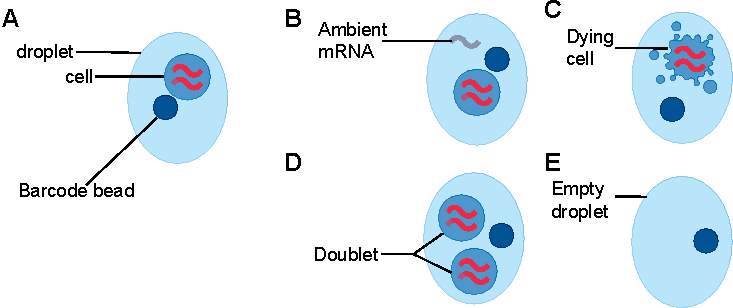
\includegraphics[width=0.95\textwidth]{PHLOWER_schematic/fig}
    \vspace{0.1cm}
    %\caption[Schematic overview of major steps of PHLOWER.]{xxxx}
    \caption[Schematic overview of major steps of PHLOWER.]{\textbf{Schematic overview of major steps of PHLOWER.} PHLOWER receives as input a multimodal or unimodal single cell data. \textbf{A)} It next creates a graph representation and a graph embedding (kamada-kawai algorithm) of the cells. Our example is based on a differentiation system of mouse embryonic fibroblasts (MEF) towards neurons or myocytes~\citep{treutlein2016dissecting}. From this graph, PHLOWER uses a zero order Laplacian decomposition and random-walk to estimate pseudo-time from progenitor cells (i.e. MEF). \textbf{B)}, Next, a simplicial complex (SC) is obtained by Delaunay triangulation of the graph represented in the kamada-kawai embedding and connecting cells end state cells with progenitor cells \textbf{C)} An edge embedding is obtained via the decomposition of the Hodge-Laplacian. In the MEF data, the first two eigenvectors have zero eigen-vectors and their signals discriminate edges belonging to the two differentiation trajectories (or holes in the SC). \textbf{D)} PHLOWER performs next random walks to obtain trajectories and uses the HL decomposition to obtain a trajectory embedding and a cumulative trajectory embedding. Clustering analysis in the trajectory embedding reveals major trajectories in the data, while the cumulative embedding space is used to estimate trajectory backbones and branching points events. PHLOWER outputs stream trees representing the differentiation tree over pseudo-time and allow the detection of regulators and gene markers.}
    \label{fig:PHLOWER_schematic}
\end{figure}

PHLOWER requires, at a minimum, dimensional reduction as input as well as a count matrix to be processed by itself. The output of PHLOWER is a STREAM tree as visualization that shows the cell differentiation tree. In addition, PHLOWER outputs a tree structure with detailed random walk paths for downstream analysis.

By default, PHLOWER is designed to work seamlessly with Scanpy and Episcanpy. It also offers a range of analysis methods for cell differentiation downstream. For example, `phlower.tl.tree\_mbranch\_markers' is used to find significant markers for each branch against the rest of the branches. Moreover, for multimodal data, such as single-cell transcriptome and open chromatin, one can call `phlower.tl.branch\_TF\_gene\_correlation' to correlate two features along tree branches. With this, one can create a heatmap matrix using the function `phlower.tl.branch\_heatmap\_matrix' to show the features along the trajectories.


% python package dependencies
\begin{table}[!ht]
	\centering
	\begin{tabular}{lll}
		\toprule
		\textbf{Package} & \textbf{Version} & \textbf{Website} \\
		\midrule
			Numpy& >=1.23.5 & \url{https://numpy.org/} \\
			Matplotlib& >=3.6.0 & \url{https://matplotlib.org/} \\
			Seaborn& >=0.12.0 & \url{https://seaborn.pydata.org/} \\
			Pydot& >=1.4.2 & \url{https://github.com/pydot/pydot} \\
			Igraph& >=0.10.5 & \url{https://igraph.org/python/} \\
			Scikit-learn& >=1.1.2 & \url{https://scikit-learn.org/stable/} \\
			Scipy& >=1.10.1 & \url{https://www.scipy.org/} \\
			Pandas& >=1.3.5 & \url{https://pandas.pydata.org/} \\
			Plotly& >=5.13.1 & \url{https://plotly.com/} \\
			Tqdm& >=4.64.1 & \url{https://github.com/tqdm/tqdm} \\
			Leidenalg& >=0.9.1 & \url{https://github.com/vtraag/leidenalg} \\
			%louvain& >=0.8.0 & \url{} \\
			Colorcet& >=3.0.1 & \url{https://github.com/holoviz/colorcet} \\
			Umap-learn& >=0.5.3 & \url{https://github.com/lmcinnes/umap} \\
			Scikit-sparse& >=0.4.8 & \url{https://github.com/scikit-sparse/scikit-sparse} \\
			Scanpy& >=1.9.3 & \url{https://github.com/scverse/scanpy} \\
			Anndata& >=0.8.0 & \url{https://github.com/scverse/anndata} \\
            Magic-impute & >=0.8.03.0.0 & \url{https://github.com/KrishnaswamyLab/MAGIC}\\
		\bottomrule
	\end{tabular}
	\vspace{0.1cm}
	\caption[PHLOWER tool python package dependencies]{PHLOWER tool python package dependencies.}
	\label{tab:phlower_python_dependencies}
\end{table}
% a table shows the python dependencies
% check how to rotate the title text of a table, see Li's table 3.2

To ensure users utilize PHLOWER correctly, we have deployed PHLOWER documents to \url{https://phlower.readthedocs.io/en/latest/}, where one can easily check the vignette for using PHLOWER, as well as the API.

We have tested PHLOWER with Python (3.8-3.10) and required dependencies, such as Numpy 1.23.5, Matplotlib 3.8.1, Seaborn 0.13.0, Pydot 1.4.2, Igraph 0.10.5, Scikit-learn 1.1.2, Scipy 1.10.1, Pandas 2.0.3, Plotly 5.13.1, Tqdm 4.64.1, Leidenalg 0.9.1, Louvain 0.8.0, Colorcet 3.0.1, Umap-learn 0.5.3, Scikit-sparse 0.4.8, Episcanpy 0.4.0, Scanpy 1.9.3, Anndata 0.9.2, Magic-impute 3.0.0.

We executed PHLOWER on a local Linux Mint 21.1 x86\_64 64-bit machine with 12 Intel(R) Core(TM) i5-10400 CPUs at 2.90GHz and 64 GB RAM. Additionally, we ran PHLOWER on a High-Performance Computing (HPC) cluster primarily based on AMD EPYC 7452 64-bit nodes at 2.35 GHz and 500 GB RAM with Rocky Linux 8.9.

For more information about PHLOWER implementation, source code, tutorials and examples, please see:
\begin{center}
\url{https://github.com/CostaLab/phlower}
\end{center}

\section{Discussion}
\label{TI_methods:discussion}
In this chapter, we discussed our computational methods for single-cell multimodal trajectory inference. We first introduce, next xxx
Finally, we described the implementation details(sref{})

From a conceptual standpoint, when comparing our method of Hodge Laplacian decomposition with competing methods, it becomes evident that the latter either connect clusters to derive trajectories or identify backbones in low dimensions (2,3) to represent trajectories. However, none of these methods effectively utilizes the high dimensions of a graph for inference. In contrast, our method utilizes edges in the high-dimensional cumulative trajectory space to identify branching points. This marks the first time Hodge Laplacian decomposition is employed to create a tree structure. Such innovation can find applications not only in biology but also in areas such as traffic detection and beyond.

\begin{itemize}

    \item We emphasized the utilization of high-level graph information, specifically the Hodge Laplacian, to capture not only relations between vertices and edges but also relations between edges and triangles. Leveraging more information allows us to derive more accurate trajectories for single-cell analysis.

    \item Subsequently, we developed a trajectory inference method based on the decomposition of the Hodge Laplacian. Our approach goes beyond a simple application of this theory to the single-cell trajectory inference problem. Incorporating essential elements such as hole creation and triangulation tricks, we address the nuances of the problem. Additionally, to overcome the issue of preference random walk getting stuck in local areas, we propose a two-step process. First, we perform the walk on the diffusion graph, followed by finding the shortest paths on the triangulated graph. The creation of a tree structure is also crucial, and we achieve this by calculating normalized distances for edges in the cumulative trajectory space to determine branching points

\end{itemize}


